\subsection{Budowa protokołu ZigBee}

\par
\tab \textbf{Opis protokołu} \\
 Jak wcześniej wspomniano ZigBee jest protokołem definiującym zasady komunikacji dla energooszczędnych urządzeń zasilanych jedną baterią przez wiele lat. \\
\tab Aby dobrze rozumieć sam protokół trzeba zrozumieć jego zastosowanie obok takich interfejsów komunikacyjnych jak Bluetooth czy Wi-Fi. Zigbee jest protokołem który może mieścić się praktycznie w każdym krzemowym układzie o wielkości kilkunastu mm i po dołączeniu anteny oraz baterii działać kilka lat bez potrzeby łądowania czy podłączania do zewnętrznych układów. Ze względu na te cechy Zigbee nie jest odpowiednim protokołem do zastosowań wszędzie tam gdzie odbywają się transfery dużych danych. \\

\par
\tab \textbf{Budowa warstwowa ZigBee} \\ 
Tak jak w przypadku wszystkich protokołów komunikacyjnych mamy tu doczynienia z wielowarstwowością. W poprzednim rozdziale została omówiona zależność między protokołem ZigBee a standardem IEEE 802.15.4 oraz omówione najniższe warstwy  protokołu: PHY oraz MAC, z tego powodu w tym rozdziale zajmiemy się jedynie warstwami wyższymi które są zdefiniowane przez standard ZigBee i są jego integralną częścią. \\
Standard definiuje dwie główne warstwy: sieciowa NWK oraz aplikacji APL.  \\

\centerline{ 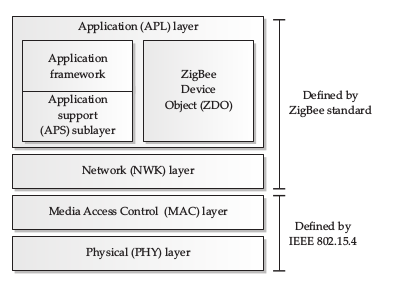
\includegraphics[scale=0.60]{./img/zigbee_layers.png} }

\par
\tab Warstwa sieciowa NWK\\
Warstwa sieciowa jest odpowiedzialna za formowanie sieci, odkrywanie urządzeń, alokacje adresów sieciowych czy ruting. \\
\tab Formowanie sieci jest procesem w którym urządzenie  tzw FFD (Fully Functional Device - czyli nie Sleeping End Device) zakłada własną sieć czyniąc się koordynatorem sieci. Wybiera ono również odpowiedni kanał częstotliwościna którym następuje transmisja w danej sieci oraz jest ustalana unikalna wartość PAN ID która nie może kolidować z innymi sieciami. \\
Kiedy sieć zostanie już ustalona Koordynator może zezwalać innym urządzeniom na dołączenie do sieci. Kiedy nowy węzeł dołącza do sieci Koordynator przedziela mu unikalny 16-bitowy adres NWK. \\

\par
\tab Warstwa aplikacji APL\\
Jest to najwyższa warstwa protokołu ZigBee, która definiuje operacje oraz interfejs funkcjonalny dla urządzenia, oraz obiektów należących do protokołu ZigBee. Obiekty te są zdefiniowanymi przez ZigBee Alliance jako standardowe profile oraz implementowane na poziomie APL używane do komunikacji z niższymi warstwami protokołu. Pojedyńcze urządzenie może implementować do 240 różnych obiektów. \\
Podstawowym elementem jest tzw. \textit{ZigBee Device Object ZDO} który jest to odpowiedzialny za dostarczenie funkcjonalności wymaganych przez wszystkie inne części protokołu oraz również za rolę urządzenia (Koordynator, Ruter, End Device), czy również za funkcjonalności związane z bezpieczeństwem takie jak kryptografia, zarządzanie kluczami. \\
\tab W skład APL wchodzi również podwarstwa APS (Application Support Sublayer) która pełni rolę łącznika między aplikacją a warstwą sieciową uwzględniającą przedewszystkim profil urządzenia. Przykładowo z punktu widzenia warstwy APS transfer danych za pomocą protokołu ZigBee nie kończy się na przekazaniu ramki danych do niższej warstwy a również czekanie na potwierdzenie od urządzenia docelowego czy dalsze przekazanie pakietu w ramach rutingu. \\

\par
\tab \textbf{Profile ZigBee} \\
Jako dodatkową cechę standardu ZigBee ułatwiającą realizację aplikacji opartych o ten standard ZigBee Alliance wprowadziło profile dotyczące różnych zastosowań przemysłowych. Ma to na celu zdefiniować standardowe wymagania oraz narzucić dobre praktyki w implementacji sieci oraz również dostarczyć narządzia i metodyki testowe czy możliwość certyfikacji całego układu. \\

Przykładowe profile ZigBee:
\begin{enumerate}
	\item Commercial Building Automation (CBA) : Profil dotyczący automatyki budynków przemysłowych
	\item Home Automation (HA) : Profil dedykowany do automatyki domowej w zastosowaniach prywatnych
	\item Health Care Profile (HCP) : Dedykowany dla urządzeń medycznych
 	\item Smart Energy Profile (SEP) : Profil stworzony z myślą o energooszczędnych systemach sensorów.
\end{enumerate} 

\clearpage